\section{Lifecycle}
\subsection{Transport}
In diesem Abschnitt wird betrachtet welchen Weg eine Flasche von Kalifornien zurücklegt bis bei einem Einzelhändler in Konstanz im Regal entsteht. Hauptaspekt in dieser Betrachtung ist der entstandene Co2 Ausstoss pro Flasche Wein. Grundlage hier dient eine Untersuchung der Justus-Liebig-Universität in Gießen (JLU). 
\begin{description}
	\item[1 Station]\hfill \\
	Flaschenabfüllung beim Weinbaubetrieb in Acampo, San Joaquin County, 			Kalifornien und sechs Kilometer Transport per LKW (Beladung mit 4.704 			Flaschen) zum Ravenswood-Distribution-Center in Lodi, San Joaquin 				County, Kalifornien
	\item[2 Station]\hfill \\
	Beladung eines 20-PANAMAX-Containers mit insgesamt 12.768 Flaschen 			und 140 Kilometer LKW-Transport des Containers zum Port of Oakland, 			Kalifornien.
	\item[3 Station]\hfill \\
		17.283 Kilometer Seetransport des Containers von Oakland über Panama 			zum Europoort Rotterdam, Niederlande;
	\item[4 Station]\hfill \\
		Umladung des Containers auf ein Rheinschiff und 487 Kilometer Transport 			nach Mainz sowie	
	\item[5 Station]\hfill \\ 
	152 Kilometer LKW-Transport des 20-Fuß-Containers von Mainz bis zum 			Weinhändler nahe Koblenz
\end{description}

Ergebnis einer Studie der Justus-Liebig-Universität Gießen (JLU) in Kooperation mit der San Francisco State University: Der globale Transport einer Flasche kalifornischer Wein über 18.000 Kilometer vom Abfüller in Kalifornien bis zum Einzelhandel gerade einmal 200 Gramm Kohlendioxid zuzurechnen. 200 Gramm Kohlendioxid werden beispielsweise frei, wenn ein privater PKW eine Strecke von nur 1,4 Kilometer zurücklegt.  (Kohlendioxid-Bilanz für kalifornischen Wein überraschend gut — (Justus-Liebig-Universität Gießen,2015). 


CO2 Ausstoss bei der Produktion
Bei der Produktion von Wein fallen durch verschiedene Arbeitsprozesse CO2 Emissionen an. Solche Arbeitsprozesse sind z.B Beschaffung und Verteilung von Dünger mit einem Traktor, Transport der Arbeitskräfte an den Einsatz Ort, Abtransport der Ernte. All dies sind Faktoren die einen unter anderem einen Ausstoss von Kohlendioxid zur Folge haben. In der Schweiz liegt dieser Wert pro ein Kilogramm produzierten Weintrauben zwischen 0.45 kg CO2-eq/Falsche und 0.6 kg CO2-eq/Falsche (ADEME, 2015). Die Variation entsteht durch die verschiedenen Traubensorten welche angebaut werden. In Kalifornien liegt dieser Wert bei 0.3 kg CO2-eq/Falsche bei der Lodi Sorte und bei 0.675 kg CO2-eq/Falsche bei der Napa Sorte.
Anhand dieser Zahlen kann man sagen das der Wein welcher in Kalifornien produziert wird ein bisschen weniger umweltbelastend ist als solcher in der Schweiz. Als Konsument muss sollte man aber beachten das der Wein aus Kalifornien durch seine lange Reise noch um die 0.2 kg CO2-eq/Falsche dazukommen. Dieser Wert ist entgegen der Erwartung eher klein, dies liegt daran das die Weinflaschen hauptsächlich im grossen Verbund auf einem Containerschiff den Grossteil der Strecke zurücklegen.Dazu kommt das nur ein nur ein kleiner Prozentsatz(unter 2\%) des Schweizer Weines exportiert wird und der grossteil direkt in der Schweiz verwertet wird. Die dadurch verursachten Emissionen sind dadurch minimal. 

\subsection{Löhne}
\subsubsection{Schweiz}
In der Schweiz sind die Lebensgrundkosten sehr hoch, und dafür ist es wichtig dass die Arbeiter angemessen bezahlt werden um zu gewährleisten dass ein gewissen Lebensstandard einzuhalten. Unter dem Motto "Ein glücklicher Mitarbeiter ist ein produktiver Mitarbeiter " werden in der Schweiz gemäss
(„Branchenverband Deutschschweizer Wein“ , 2016) auch anständige Löhne für die hiesigen Mitarbeiter bezahlt. Mit einem Einstiegslohn von rund 4700 werden Winzer auch für die körperlich anstrengende Arbeit gerecht entlohnt. Durch das schweizerische Dreisäulensystem dient als angemessene Sicherung des Existenzbedarf und gilt als Sicherheit für die Arbeiter. Im ganzen gesehen ist der Beruf des Winzers in der Schweiz als sicher zu betrachtet.

\subsubsection{Kalifornien}

Der durchschnittliche Verdienst in den Vereinigten Staaten von Amerika beträgt rund um die 3080 US Dollar pro Monat. (Quelle: Erhebung des US Census) Dieser Betrag schwankt ein wenig von Staat zu Staat, aber dient hier nur als Vergleich. Bezüglich des Verdienstes spielt es in der kalifornischen Weinproduktion eine essenzielle Rolle welchen Beruf ausgeübt wird. So verdient ein sogenannter «Winemaker», was der Chef einer Kellerei ist, um die 9000 US
Dollar und ein Assistent um die 5 730 US Dollar pro Monat. Diese Werte liegen beide ziemlich weit über den weiter oben genannten Nationalen Durchschnitt. Zu beachten gilt hier dass nur wenige Personen diese Berufung pro Kellerei ausüben. Der Grossteil der Arbeit
wird von sogenannten «grape picker» verrichtet. Diese Pflücken die Weintrauben auf dem Feld. Ein solcher Feldarbeiter verdient im Durchschnitt circa 10 US Dollar pro Stunde,
\cite{_farm_????} hochgerechnet auf ein pro Monat macht das 1500 US Dollar, dies ist um einiges weniger als der Durchschnitt. Die harte Feldarbeit wird zu einem grossen Teil von mexikanischen Immigranten verrichtet, ähnlich in Spanien bei welchen die Feldarbeit von polnischen Immigranten verrichtet wird.
  \begin{figure}[H]
	\centering
	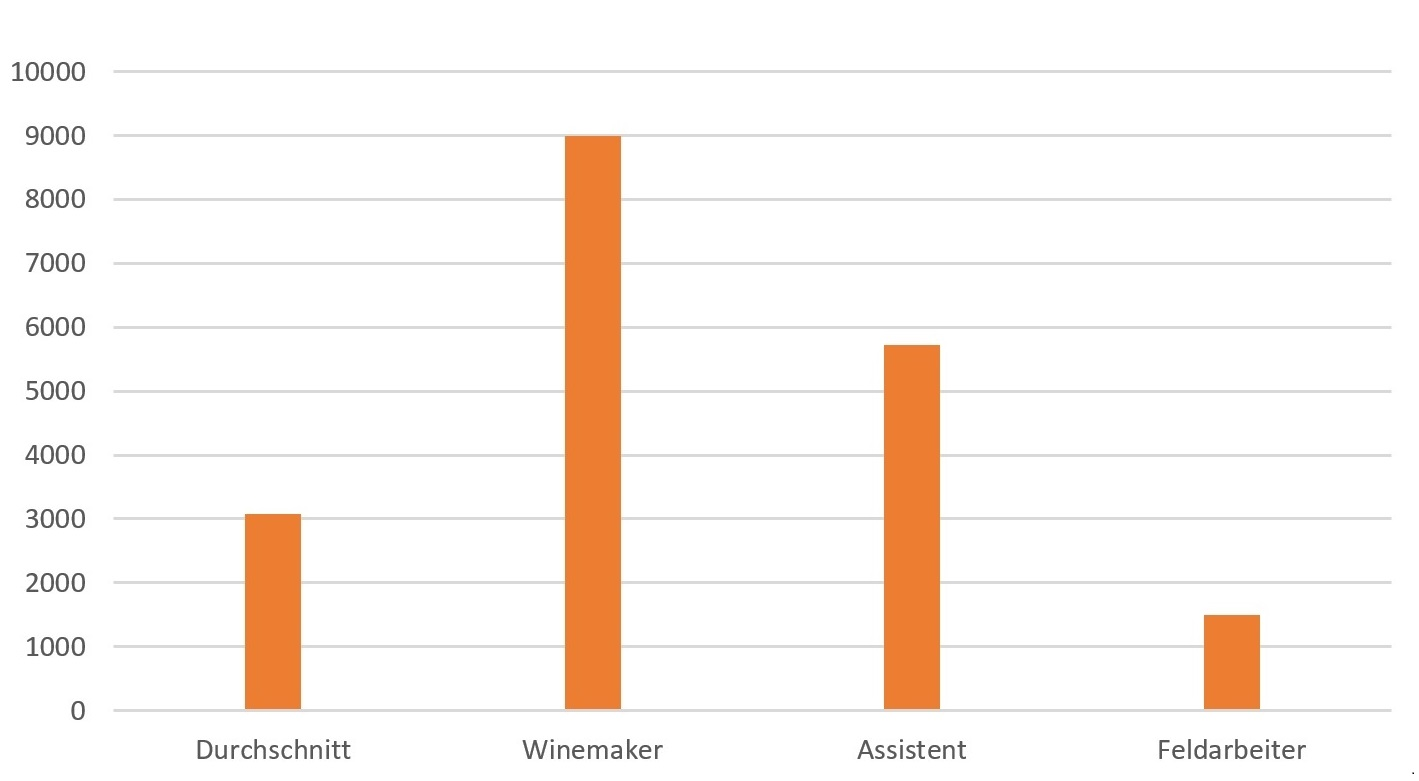
\includegraphics[width=0.9\textwidth]{Grafikarbeiter}
	\caption{Löhne der Arbeiter in der Weinproduktion}
\end{figure}
Die Arbeitsbedingungen in der USA sind im Verhältnis zur Schweiz rückständig, so hat ein Arbeitnehmer in den USA praktisch keinen Kündigungsschutz. Dies liegt an der grossen Mobilität an den Amerikanern. Die amerikanischen haben aber Anspruch auf eine Rente, welche sie ähnlich der Schweiz mit ihrem Lohn bezahlen. \cite{_arbeitszeiten_????} Wie man unschwer erkennt ist das ein Feldarbeiter in Kalifornien unterbezahlt. Hier liegt auch ein grosses Verbesserungspotenzial. Ein gerechter MIndestlohn der per Gesetz geregelt ist, ähnlich wie in der Schweiz, würde die Lage für viele der Feldarbeiter stark verbessern. Du beachten ist dass ein Feldarbeiter im Schnitt nur ein Monat auf den Feldern arbeitet, so ist eher eine Temporäre Anstellung und eine Gesetzgebung könnte sich als schwer gestalten, denn je nach Ernte und Jahr  müssen die Winzer flexibel reagieren können.


\subsection{Wasser}
\subsubsection{Kalifornien}
\label{sub:wasserverbrauch}

In Kalifornien werden etwa 42'000 $m^3$ Wasser für die Landwirtschaft benötigt. Das entspricht  39 \% des gesamten
Wasserverbrauchs. 

Der Wasserverbrauch beim Weinanbau ist grundsätzlich nicht so hoch wie bei anderen Pflanzen. Es
werden dennoch rund 700 Liter Wasser pro Liter Wein benötigt.
(\glqq{}The Water Footprint of the Wine Industry\grqq{} (2015)). 

In Kalifornien
herrscht seit 2011 eine Dürre, die Wasserrationierung nötig machte. Daher regulieren über 90 \% der
Weingüter aktiv ihre Bewässerung. Die grösste Einsparung gibt es durch die Tropfbewässerung. Dabei
wird das Wasser direkt den Wurzeln  des Weinstocks zugefügt. Dabei verdunstet weniger Wasser
unbenutzt.

Zusätzlich fliesst auch kein Wasser ab und es werden keine Nährstoffe ausgeschwemmt. Das reduziert
den Einsatz von Dünger und die Eutrophierung des Grundwassers.

Wo es der Untergrund zulässt, wird auf Trockenfeldbau gesetzt.

(\glqq{}California Wine Community Sustainability Report Appendix\grqq{} (2015)).


Auch bei der Produktion in den Kellereien wurde Massnahmen getroffen, um das verwendete Wasser zu
reduzieren. Hier fällt es vor allem für die Reinigung der Gärtanks an. Dieses Wasser wird nun
aufgefangen und wiederverwendet.


\subsubsection{Schweiz}
Die Schweiz wird oft als das Wasserschloss von Europa bezeichnet. «Viele wichtige Flüsse Europas – Rhein, Rhone, Inn (Donau) und Tessin (Po), Etsch (Adige) – nehmen ihren Ursprung hierzulande. Obschon die Schweiz flächenmässig nur knapp vier Promille am Kontinent ausmacht, befinden sich auf ihrem Boden sechs Prozent der Süsswasservorräte Europas». („Wasserschloss Schweiz - NZZ“, o. J.)
 \begin{figure}[H]
	\centering
	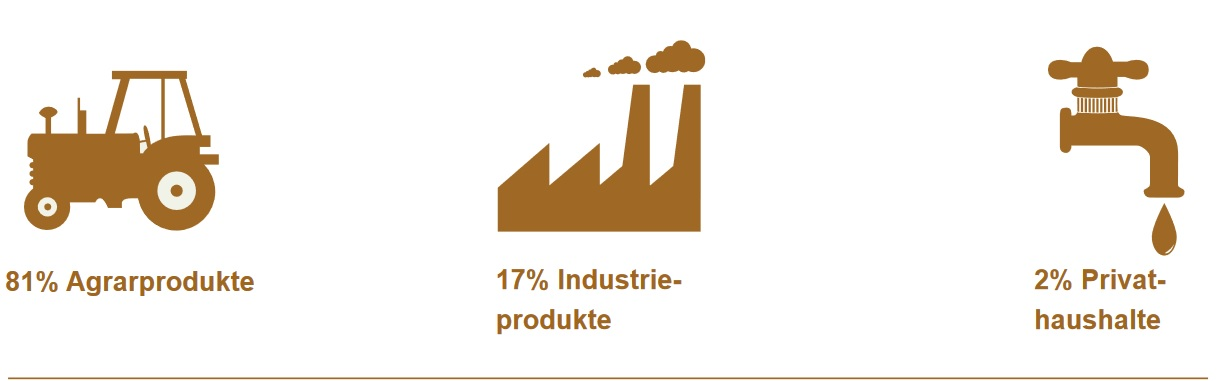
\includegraphics[width=0.9\textwidth]{WV}
	\caption{Wasserverbrauch aufgeteilt nach Sektoren}
\end{figure}
 Der Gesamtwasserverbrauch in der Schweiz liegt bei 1960 Mio. $m^3/Jahr$ dieser Verbrauch teilt sich auf auf die Privathaushalte (2\%), Industrie (17\%) und auf den Agrarsektor (83\%) auf. Die Wein und Bierproduktion braucht hierzulande nur 3\% des Agrarwasserverbrauchs. Für die Weinproduktion muss in der Schweiz nur sehr wenig Wasser eingesetzt werden, da die Niederschläge meistens ausreichen. (Wettstein u. a., 2016)
  \begin{figure}[H]
	\centering
	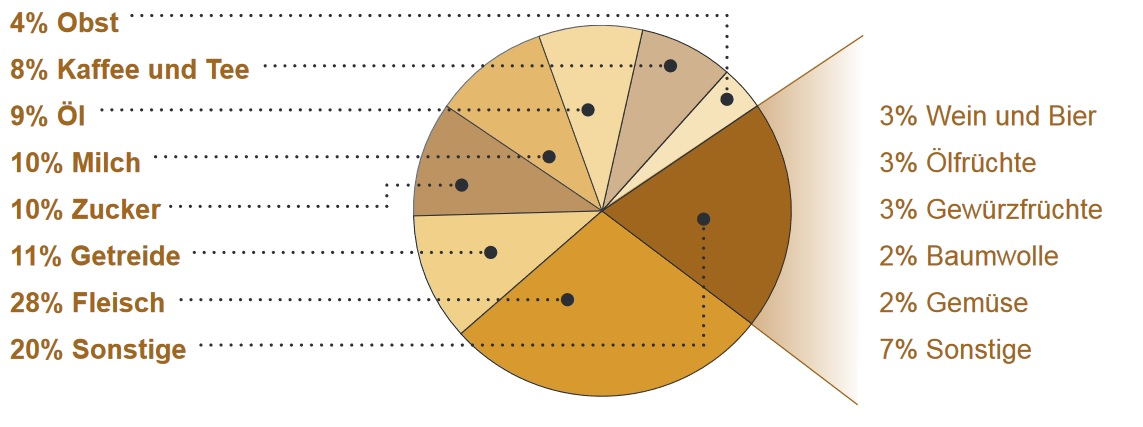
\includegraphics[width=0.9\textwidth]{WVA}
	\caption{Anteile des Wasserverbrauchs im       Agrarsektor}
\end{figure}
 
  Durch die grosse Verfügbarkeit und die geringe Nutzung von Wasser für den Weinbau ist der Wasserverbrauch für Wein in der Schweiz nicht problematisch. Jedoch sind die Wasserverschmutzungen die durch die Weinproduktion entstehen nicht unproblematisch. Zur Wasserverschmutzung tragen vor allem Ausschwemmungen von Pestiziden bei.
  \newpage
\subsection{Pestizide}
Dieser Abschnitt befasst sich um die Umweltbelastung durch Pestizide. Ein Winzer ist darauf angewiesen die Ausfälle der Ernte möglichst klein zu halten um sein Lebensunterhalt zu finanzieren. Ein grosser Anteil der Ausfälle ist auf Schädlinge zurückzuführen. Um Schädlinge von der Traube fernzuhalten, wird immer wieder auf Pestizide vertraut. Dieses Verhalten bringt sofort die Frage hervor ob durch den Einsatz von Pestiziden immer noch umweltfreundlich und nachhaltig produziert werden. Wie in diesem Abschnitt aufgezeigt wird gibt vor allem grosse Unterschiede ob ein Wein nach Bio oder ÖLN Standards Produziert wird.
\subsubsection{Schweiz}
\begin{wrapfigure}{r}{10cm}
	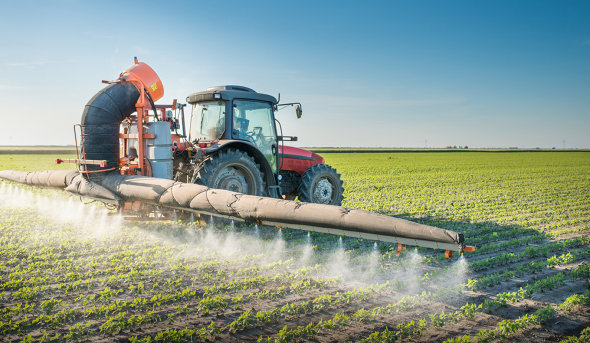
\includegraphics[width=9.5cm]{pestizide}
	\caption{Pestizide werden auf dem Feld verteilt.}
\end{wrapfigure}
In einer umfassenden Studie wurde von Greenpeace Schweiz sechs Weinberge in verschiedenen Weinbauregionen auf Pestizide untersucht. Insgesamt wurden 33 Wirkstoffe festgestellt von den 23 auf der Greenpeace "Blacklist" welches bedeutet diese Wirkstoffe sind entweder humantoxisch oder haben eine inakzeptable Wirkung auf das Ökosystem. Zwei der gefunden Wirkstoffe waren sogar durch die EU nicht zugelassen. In den Böden konnten ältere Pestizide nachgewiesen werden, welches aufzeigt das sich manche Pestizide nur sehr langsam abbauen und über Jahrzehnte Schäden in den Ökosystemen anrichten. In der Studie wurden auch die fertigen Weine auf ihre Inhalte überprüft. In der konventionellen Weinprodukten wurden vermehrt Rückstände von Pestiziden gefunden , welche aber die Grenzwerte nicht überschreiten. Allerdings gibt es für Weine auch nur selten Pestizid Grenzwerte.Wie in Abbildung \ref{fig:ha} dargestellt, ist die UBP von ÖLN ein wesentlicher Bestandteil der gesamten Belastung. Der Unterschied zur biologischen Produktion wird deutlich, die eine Anwendung von Pestiziden verbietet.
 \begin{figure}[H]	
	\centering
	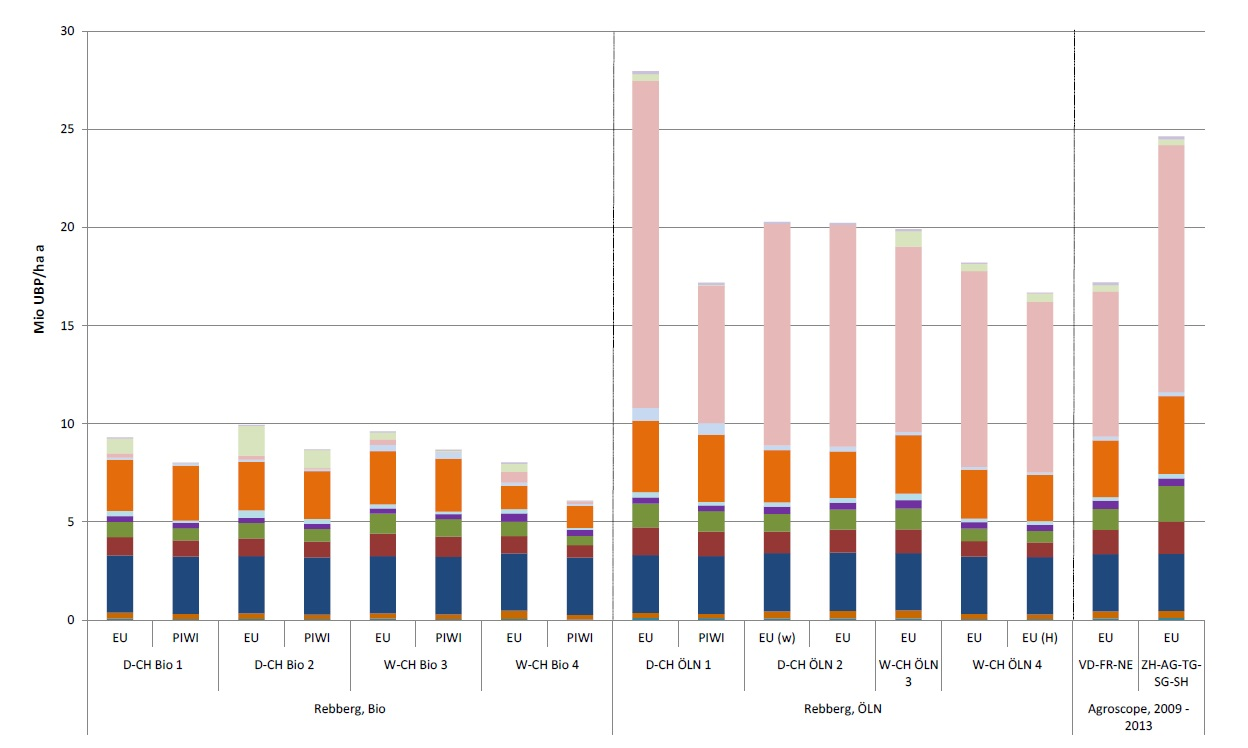
\includegraphics[width=0.9\textwidth]{auswirkungen}
	\caption{Gesamtumweltbelastung [UBP] der ÖLN- und biologischen Bewirtschaftung einer Hektare Rebbergs}
	\label{fig:ha}
\end{figure}

\subsubsection{Kalifornien}
\label{sub:sch_dlingsbek_mpfung}

Das Ziel der Schädlingsbekämpfung in Kalifornien ist nicht das komplette Ausrotten oder Verhindern
der Schädlinge. Es werden stattdessen Schwellenwerte definiert. Es werden erst Massnahmen getroffen,
wenn diese Schwellenwerte erreicht oder überschritten werden. Diese Massnahmen umfassen biologische,
kulturelle und chemische Mittel, die so eingesetzt werden, dass ökonomische, Umwelt- und
Gesundheitsrisiken minimiert werden.

Um den Einsatz von giftigen Pestiziden zu verringern, werden diese erst eingesetzt, wenn es wirklich
nötig ist. Das setzt eine kontinuierliche Kontrolle über den Schädlingsbefall voraus. Dies wird von
etwa drei Viertel der Weinbauern vorgenommen.

Als Prävention werden kulturelle Massnahmen getroffen. Dazu gehören das Entfernen von Laub, Hecken,
Staubkontrolle und Bewässerung.

(\glqq{}California Wine Community Sustainability Report Appendix\grqq{} (2015))
(\glqq{}California Wine Community Sustainability Report\grqq{} (2015))

Zu den biologischen Schädlingsbekämpfungsmittel gehören natürliche Feinde wie Spinnen, Marienkäfer
oder Wespen, aber auch Hühner oder Schafe, die gegen Erdraupen oder zum Mähen von Gräsern eingesetzt
werden  (\glqq{}Sustainable Winegrowing\grqq{} (2017)).  Durch diese Massnahmen werden weniger
Pestizide eingesetzt und die Artenvielfalt wird erhöht.